\subsection*{Magnetic Field Generation}

Magnetic fields were generated using a \textbf{custom-built air-core solenoid}, approximately 15 cm in length and 10 cm in outer diameter. The solenoid was densely wound with \textbf{copper wire ($\sim$1 mm diameter)}, forming an inner core of approximately 5 cm. A \textbf{Pasco Scientific SF-9584 DC power supply} was used to deliver currents in the range of \textbf{0--4 A}, corresponding to magnetic field strengths from \textbf{1 to 18.9 Gauss} for this solenoid. The system operated in a continuous mode; no rest periods were applied between trials due to the time required to stabilize the pendulum after each adjustment. 

\subsection{Magnetic Field and Gradient Mapping Platform}

Magnetic field strength ($B_0$) and gradient ($\nabla B_0$) measurements were performed using a commercial Gaussmeter (Model GM2, AlphaLab Inc., Salt Lake City, UT).  The GM2 operates on the Hall effect principle, wherein a voltage is generated across a probe when exposed to a perpendicular magnetic field. This voltage is proportional to the local magnetic flux density, enabling precise spot measurements of field magnitude. The Gaussmeter used has an accuracy of 1\% of the DC reading in the 16$^\circ$C to 29$^\circ$C range.

To ensure spatial accuracy and reproducibility, a fixture made from rigid \gls{pvc} was constructed by previous Creighton University students \cite{haddixProposal}. The platform comprises a 300 mm square base and a 280 mm diameter vertical circular plate, perforated with a 5x5 grid of probe-access holes spaced at 20 mm intervals as shown in figure \ref{fig:fieldmapping}. Each access point was numerically indexed to facilitate 2D field mapping in the X-Y plane.

\begin{figure}[H]
	\centering
	\begin{minipage}[t]{0.48\textwidth}
		\centering
		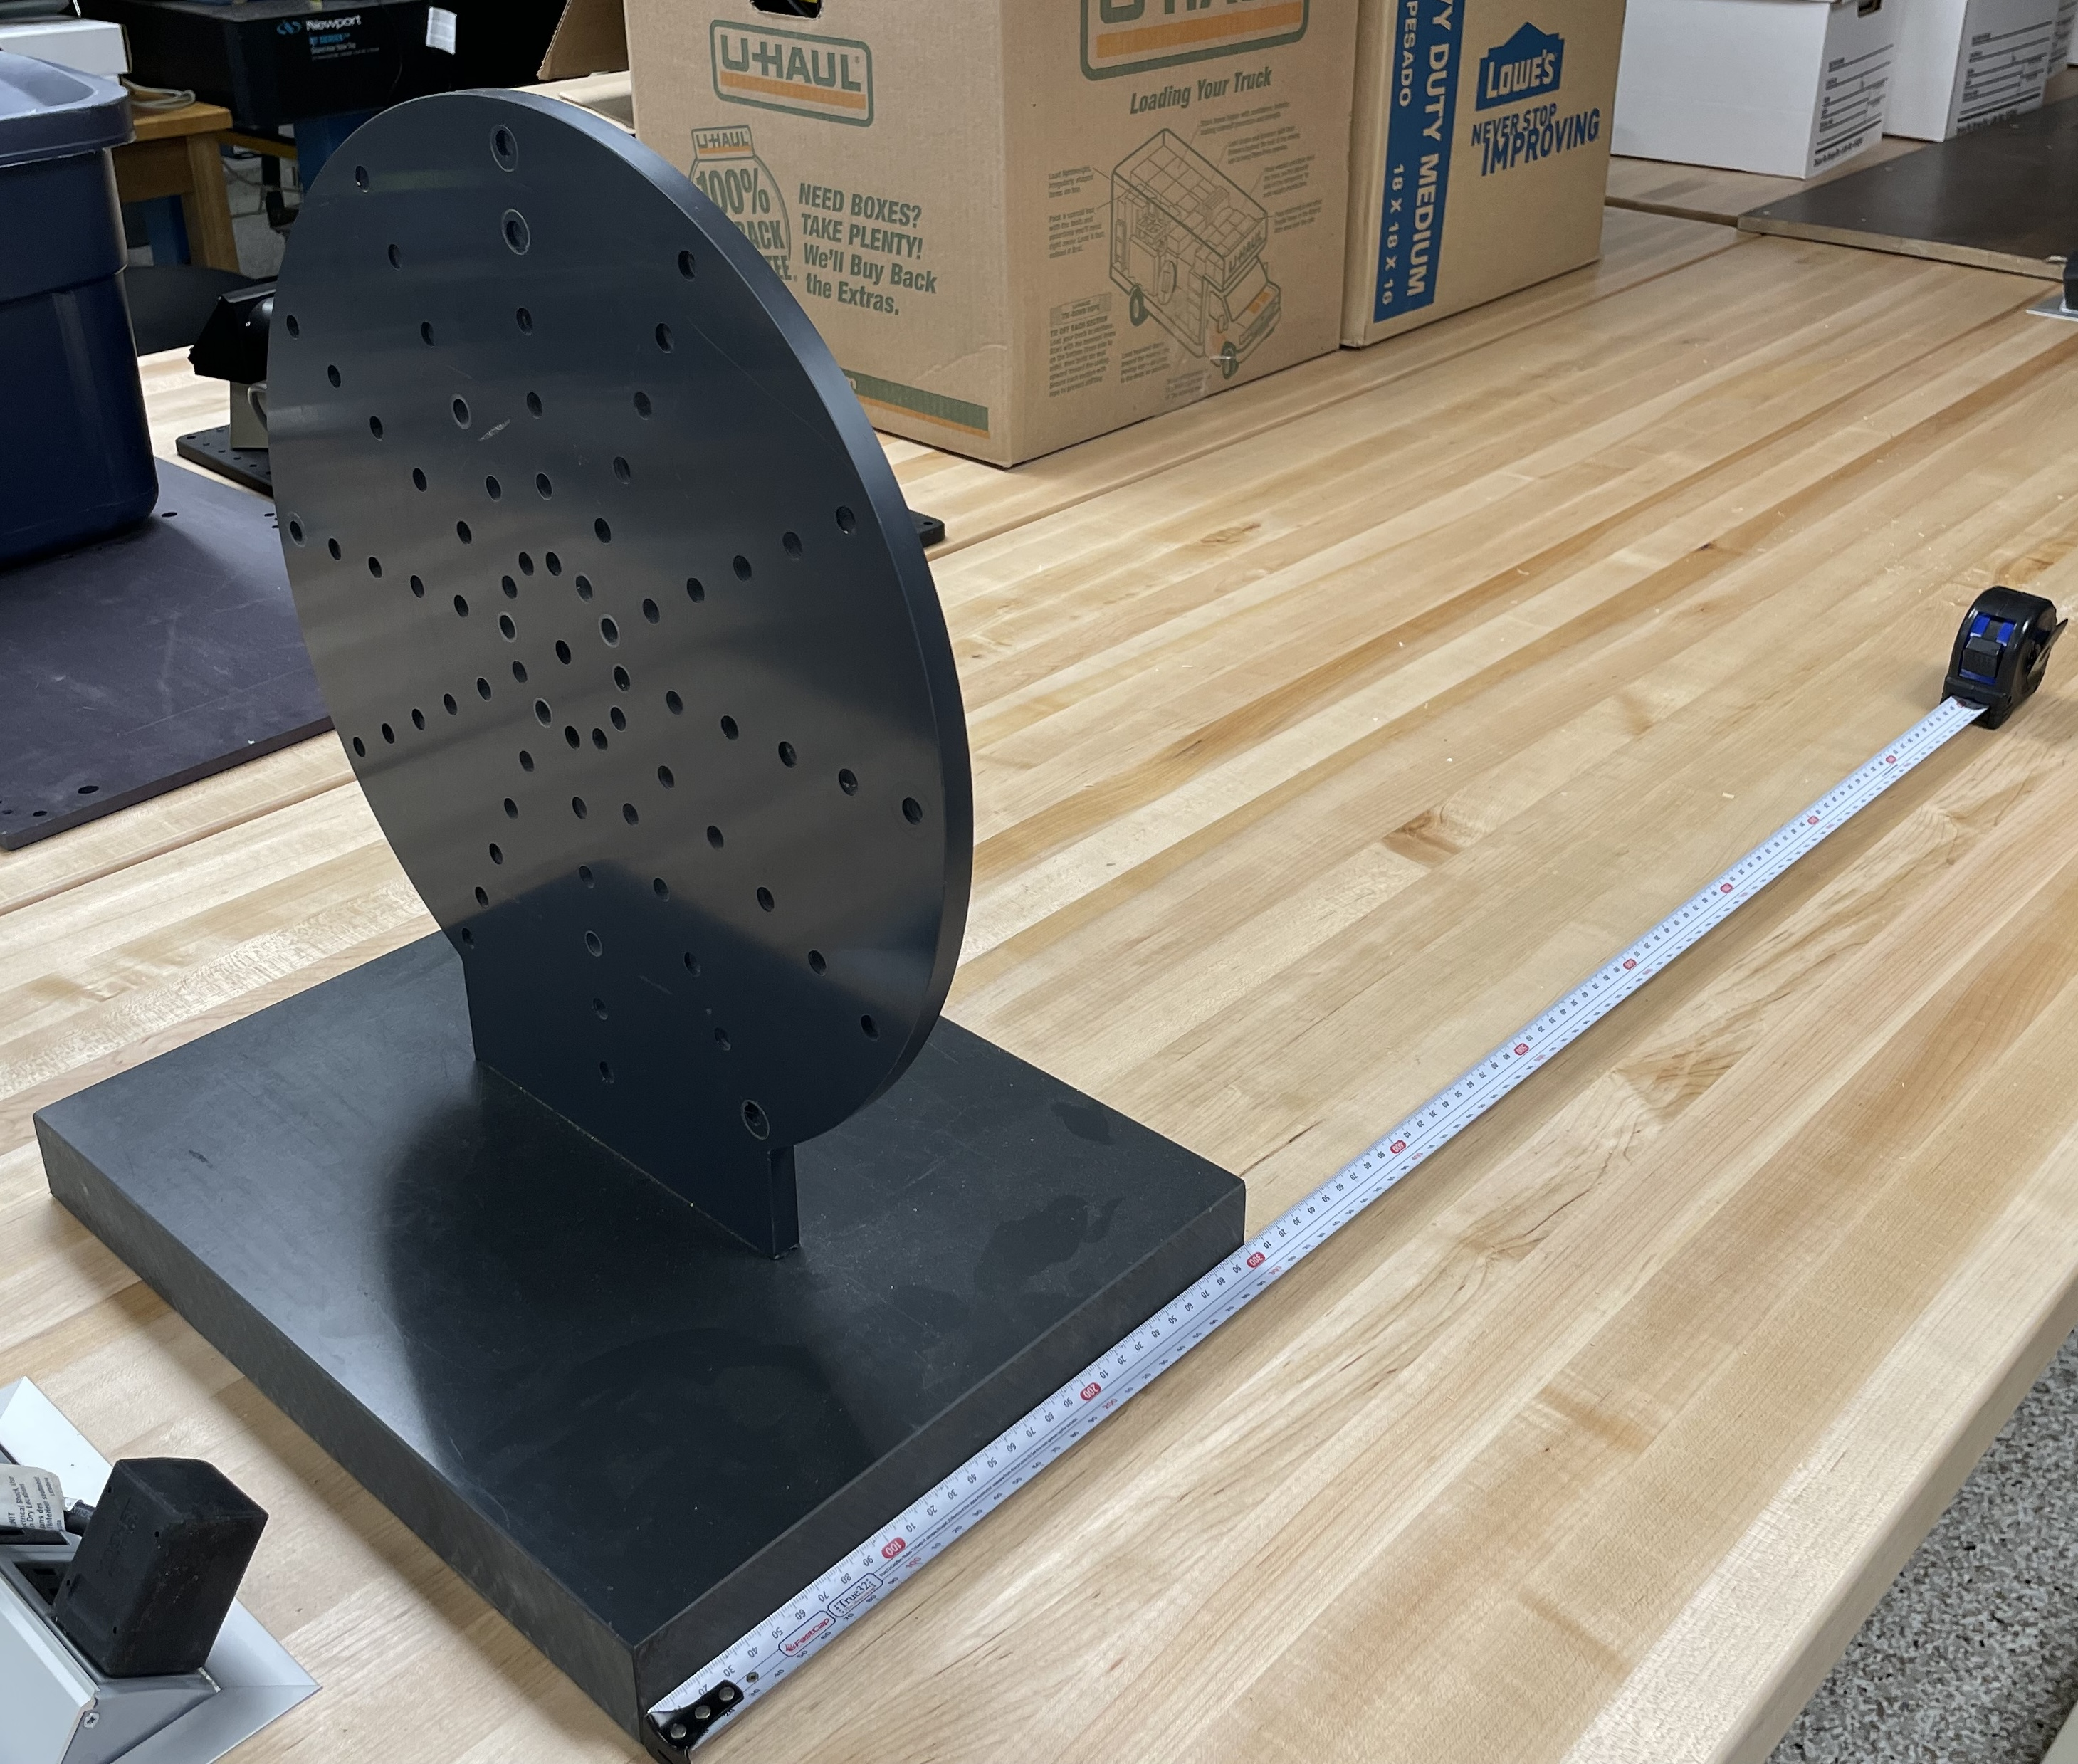
\includegraphics[width=\textwidth]{Assests/Picture3.jpg}
		\caption*{(a) PVC-based mapping platform.}
	\end{minipage}%
	\hfill
	\begin{minipage}[t]{0.48\textwidth}
		\centering
		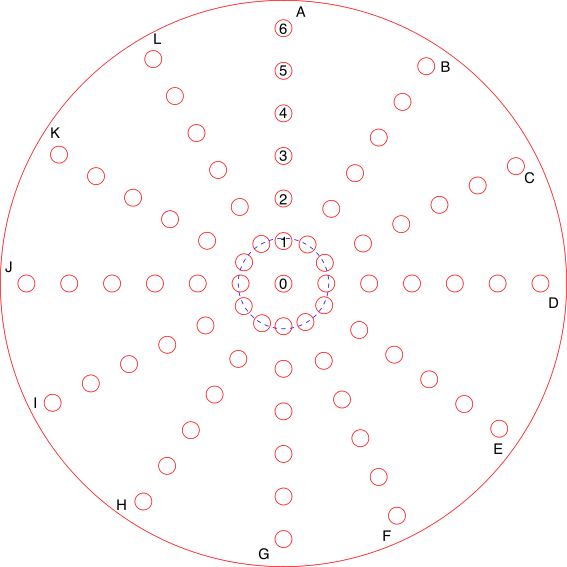
\includegraphics[width=0.85\textwidth]{Assests/MagFieldMap.png}
		\caption*{(b) Example field map output from MRI fringe region.}
	\end{minipage}
	\caption{PVC-based magnetic field mapping platform used for spatial $B_0$ and $\nabla B_0$ measurement. As shown in Ferreira 2017 \cite{haddixProposal,ferreira2017}.}
	\label{fig:fieldmapping}
\end{figure}


%LABVIEW program and Alpha Labs Protocols
Once the field‑mapping phantom and Gaussmeter probe are co‑aligned, data capture was streamlined to be sufficiently flexible and precise for our proximity measurements near an \gls{mri}. The manufacturer’s default software, AlphaApp, provides basic data‑logging, tethered or standalone recording, live screen streaming, and plotting of measurements from USB‑enabled AlphaLab meters\cite{AlphaApp}. However, AlphaApp **does not expose control over sampling frequency or allow real‑time adjustment of acquisition parameters**, limiting fine‑grained temporal resolution when the probe is moved into steep field gradients. In contrast, using \gls{lvi} interface allows for configurable sampling intervals, buffer control, and precise timing protocols, enabling us to push the device for much higher accuracy as the probe approaches and crosses isocontour regions within the \gls{mri} fringe. We developed that VI by leveraging the AlphaLab Data Acquisition Communication Protocol to command the device directly via USB, providing deterministic control over timing and sample rate \cite{AlphaAppProtocol}.

The data acquisition procedure for magnetic flux mapping is organized in this \gls{lvi}, whose basic logic is summarized in Figure~\ref{fig:gaussmeter-flowchart}. Upon startup, the \gls{lvi} initializes serial communication with the Gaussmeter, loads user-defined parameters (such as file name, mode of acquisition, delay time, and probe coordinates), and clears buffers in preparation for logging. The user may select either a continuous or an individual sampling mode. In continuous mode, the VI iterates through a defined number of data points with a fixed delay between samples; in individual mode, each data capture is triggered manually, allowing for precise positioning or timing. For both modes, each cycle involves reading the spatial coordinates, sending a measurement command, recording the returned magnetic flux value, and updating a graphical display as well as the output file.

While the flowchart reflects the core logic, it does not fully convey the customization added to the \gls{lvi} interface. For example, the front panel includes input fields for patient table (couch) parameters such as couch speed and displacement points. As mentioned above, our phantom is discretized with radial and angular indices: angular positions span 12 sectors clockwise from the 12 o’clock position (0 to 11 or A to L), and radial depths range from the center (0) to the outer edge (6). The probe’s spatial location is represented in polar coordinates, and the system plots magnetic flux as a function of position rather than time, allowing for intuitive visualization of the MRI fringe field across the phantom surface.

\begin{figure}[H]
	\centering
	\begin{tikzpicture}[node distance=1.5cm, every node/.style={transform shape}, scale=0.6]
	
	% Start
	\node (start) [startstop] {Start VI};
	
	% Initialization
	\node (initserial) [process, below of=start] {Initialize serial port (COM3, 115200 baud)};
	\node (readinput) [process, below of=initserial] {Read user inputs (file name, mode, delay, coords)};
	\node (clearbuf) [process, below of=readinput] {Clear buffers and arrays, create CSV};
	
	% Mode decision
	\node (mode) [decision, below of=clearbuf, yshift=-0.5cm] {Data collection mode?};
	
	% Individual branch: manual trigger wait before data steps
	\node (manualTrigger) [process, left=3.5cm of mode] {Wait for manual trigger};
	
	%Continuous loop
	\node (loopCount) [process, below =3cm of mode] {Loop: For i = 1 to N points};
	
	% Data acquisition steps (common)
	\node (readcoords) [process, below of=loopCount] {Read MRI coordinates (x,y,z)};
	\node (sendcmd) [process, below of=readcoords] {Send command to Gaussmeter};
	\node (readflux) [process, below of=sendcmd] {Read flux data (time, flux, error byte)};
	\node (store) [process, below of=readflux] {Append to arrays and CSV};
	\node (updateplots) [process, below of=store] {Update XY graph and polar plot};
	\node (checkerrors) [process, below of=updateplots] {Check for errors};
	
	% Continuous mode: wait delay after error check
	\node (delayWait) [process, below of=checkerrors, yshift=-1cm] {Wait preset delay};

	
	% Loop decision
	\node (moreRuns) [decision, below of=delayWait, yshift=-0.5cm] {More runs/points?};
	
	% End
	\node (end) [startstop, below of=moreRuns, yshift=-1cm] {End VI};
	
	% Arrows: initialization flow
	\draw [arrow] (start) -- (initserial);
	\draw [arrow] (initserial) -- (readinput);
	\draw [arrow] (readinput) -- (clearbuf);
	\draw [arrow] (clearbuf) -- (mode);
	
	% Mode branches
	\draw [arrow] (mode) -- node[above] {Individual} (manualTrigger);
	\draw [arrow] (mode) -- node[above] {Continuous} (loopCount);
	
	% Individual flow to data steps
	\draw [arrow] (manualTrigger) |- (readcoords.west);
	
	% Data acquisition common flow
	\draw [arrow] (loopCount) -- (readcoords);
	\draw [arrow] (readcoords) -- (sendcmd);
	\draw [arrow] (sendcmd) -- (readflux);
	\draw [arrow] (readflux) -- (store);
	\draw [arrow] (store) -- (updateplots);
	\draw [arrow] (updateplots) -- (checkerrors);
	
	% Continuous flow: after errors wait delay, then loop decision
	\draw [arrow] (checkerrors) -- (delayWait);
	\draw [arrow] (delayWait) -- (moreRuns);
	
	% Individual flow: after errors go directly to loop decision (skip delay)
	\draw [arrow] (checkerrors.east) -- ++(1,0) node[pos=0.3, right, xshift=20pt] {Individual only} |- (moreRuns.north);

	% Loop decision arrows:
	% If yes, loop back to the start of the mode branch
	% Intermediate branch point for Yes
	\node (yesBranch) [coordinate, left=2.5cm of moreRuns.west] {};
	
	% Arrow from moreRuns to yesBranch labeled "Yes"
	\draw [arrow] (moreRuns.west) -- node[midway, above] {Yes} (yesBranch);
	
	% Branch to Individual
	\draw [arrow] (yesBranch) -- node[pos=0.85,above] {Individual} ++(-7,0) |- (manualTrigger.west);
	
	% Branch to Continuous
	\draw [arrow] (yesBranch) -- node[pos=0.8,below] {Continuous} ++(-3,0) |- (loopCount.west);


	
	% If no, end program
	\draw [arrow] (moreRuns.east) -- node[midway, above] {No} ++(3,0) |- (end.east);
	
\end{tikzpicture}
	\caption{Flowchart of the Gaussmeter VI data acquisition algorithm.}
	\label{fig:gaussmeter-flowchart}
\end{figure}

In clinical use, the entire fixture is intended to be shifted axially along the Z-direction of a horizontal bore MRI scanner using controlled couch increments (e.g., 10 cm). This translation allows for volumetric sampling of $B_0$ over several planes. The spatial magnetic field gradient$\nabla B_0$ can then be estimated numerically using finite difference calculations between adjacent measurement points. This method has previously been applied to MRI mapping in the work by Ferreira \cite{ferreira2017}.



